\chapter{Introduction}
\label{sec:ch1}
 
Particle accelerators are the workhorses for modern scientific discoveries. Experimental nuclear and particle physics research benefit greatly from the progress of accelerator physics and technology. Accelerator physics is a rich field of applied physics living on the intersection of electromagnetism, solid-state and atomic physics, nonlinear mechanics, plasma physics, quantum mechanics, just to name a few \cite{sylee}. Furthermore, the design and operation of modern accelerator projects require costly enterprises of scientists, engineers, operators, and politicians coming together under one single metaphorical roof.         

The scientific principle of particle accelerators involves the acceleration, steering and/or storage of charged particles through electromagnetic manipulations. These manipulations occur through a plethora of devices and components that can control electromagnetic fields, e.g., magnets, electrical cavities. The group of particles that is subject to this electromagnetic handling is referred to as "the beam". The field of beam dynamics studies the interaction between the beam and the steering devices, as well as the Coulomb interactions between the beam itself---this is known as space charge physics. An additional distinction can be made when these steering devices are configured in a circular or linear fashion. This gives rise to the distinction between circular accelerators and linear accelerators (Linacs).

Furthermore, particle accelerators can be categorized by the type of elementary particles that compose the beam and how close to the speed of light they are traveling. The first category refers to the distinction between hadrons and leptons---particles that interact or do not interact through the strong force, respectively \cite{griffiths}. For example, protons and heavy ions are considered hadrons, while electrons and muons are considered leptons. The second category can be summarized if particles in the machine travel at a high or low energy. An example of a low-energy hadron machine is the heavy ion Linac at FRIB (Facility for Rare Isotope Beams) \cite{frib}. An example of a high-energy lepton machine was the Stanford Linear Accelerator located at SLAC National Accelerator Laboratory \cite{slac}. The two most famous high-energy hadron machines in history are the Tevatron \cite{tevatron}, which operated at Fermilab, and the LHC (Large Hadron Collider), operating at CERN \cite{lhc}. Furthermore, there are accelerator projects that encompass several categories such as the future EIC (Electron-Ion Collider) being built at Brookhaven National Laboratory \cite{eic}, which will use an electron ring---a lepton machine---and a heavy-ion circular accelerator---a hadron machine---to probe new physics. This is just to name a few. There's a plethora of accelerator projects around the world that are either operational, under commissioning or being designed. 

The following thesis will explore the beam dynamics of a circular machine used to store high-energy protons---hadrons---such as the Fermilab Recycler Ring.         

\section{Circular Accelerators and Storage Rings}

As will become more apparent on Ch. \ref{sec:ch2}, a particle accelerator can be thought of as a composition of accelerator-themed LEGO® bricks \cite{forest}. Each elemental LEGO® brick can be thought of as an accelerator component performing some mapping on the charged particles entering it. As it turns out, these LEGO® bricks can be assembled together circularly to give rise to circular accelerators. The assembly of these blocks in a particular shape gives rise to what is known as the lattice of the accelerator.

The acceleration part of these structures comes from elements inside the lattice that introduce some sort of electromotive force in the longitudinal direction. The most common example for these blocks are radio-frequency (rf) cavities \cite{sylee}, with super-conducting rf cavities also as an established technology \cite{srfcavs}. Particles that go through these elements gain energy on every pass. For the case where there are no acceleration blocks on these structures, a storage ring arises. Nevertheless, storage rings can also have rf cavities just for longitudinal beam manipulation, but no overall acceleration---such is the case of the Recycler Ring.    

Circular accelerators are special due to the fact that particles have to pass thousands or even millions of turns through the same LEGO® blocks. This gives birth to very interesting and complex dynamics inside these machines. One of these phenomena are called betatron resonances. The most simple lattice is composed of focusing and steering blocks, and they are, usually, dipole and quadrupole magnets, i.e. the lowest-order multipole magnets. For reasons that will become apparent in Ch. \ref{sec:ch2}, these elements, in combination with free drift spaces, represent linear blocks. For the simplest circular machine, these linear LEGO® bricks are assembled together to create a linear lattice. A linear lattice is designed to have stable particle orbits all around the accelerator. Nevertheless, accounted or unaccounted elements, described by linear or nonlinear blocks, around the machine can perturb the stable orbits. Ultimately, the effect of these perturbations can add up coherently over many turns to push the beam out of the acceptance of the lattice. This whole process is known as a betatron resonance in a circular accelerator. A mathematical description of this process is described on Ch. \ref{sec:ch2}.

The following thesis describes an effort to mitigate the deleterious effect of these resonances in the Recycler Ring. After dipole and quadrupole, the third order of multipole magnetic fields is the sextupole component. Therefore, sextupole fields around the lattice are the source of third order betatron resonances. Specifically, this thesis explores mitigation techniques to these third order resonances, mainly in the Fermilab Recycler Ring (see Ch. \ref{sec:ch3}, Ch. \ref{sec:ch5} and Ch. \ref{sec:ch6}), but also with some experiments done at the CERN Proton Synchrotron Booster (see Ch. \ref{sec:ch4}). 

\section{Fermilab}

The Fermi National Accelerator Laboratory (FNAL), better known as Fermilab, has a long and rich history of designing, building and operating high-energy particle accelerators. Ever since the founding director of Fermilab, Robert R. Wilson, envisioned the 400 GeV Main Ring back in 1967, Fermilab has been at the forefront of accelerator physics \cite{tevatron}.     ,\cite{fermilab1}

The current layout of the Fermilab Accelerator Complex is summarized in Fig. \ref{fig:fac}. As of 2024, the Fermilab Accelerator Complex is composed of an $H^-$ source that connects to a linear accelerator, accelerating the ions to en energy of 400 MeV. This linear accelerator feeds to the first circular machine---the Booster---where protons are achieved and accelerated to an energy of 8 GeV. After the Booster, the protons are transported to the Recycler Ring (RR), which is the second circular machine. In the RR, protons are stacked and stored in order to increase the beam intensity delivered to the Main Injector (MI). This last circular accelerator is where protons are accelerated from an energy of 8 GeV to 120 GeV. Once at this energy, the protons are transported the Neutrinos at the Main Injector (NuMI) experiment, in order to create the world's most intense neutrino beam \cite{numi1}. Nevertheless, all throughout the chain of accelerators, beam is also delivered to a plethora of other experiments being conducted at Fermilab. Therefore, the facility has several modes of operation depending on the experiments that are online. A more detailed and technical study of the current Fermilab Accelerator Complex, focusing on the Recycler Ring, is given on Ch. \ref{sec:ch3}.   

\begin{figure}[H]
    \centering
    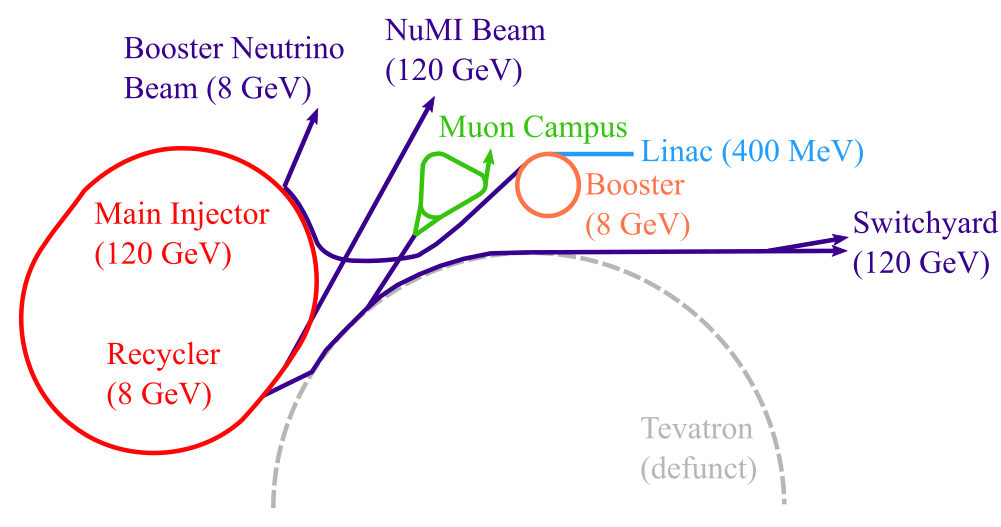
\includegraphics[width=\columnwidth]{chapter1/complex.png}
    \caption{Schematic layout of the Fermilab Accelerator Complex as of 2024. Original plot provided by R. Ainsworth.}
    \label{fig:fac}
 \end{figure}

\section{Outline}

The following thesis will explore the compensation of third-order resonances in the Fermilab Recycler Ring. \hyperref[sec:ch1]{Chapter 1} introduces the motivation behind this thesis work. \hyperref[sec:ch2]{Chapter 2} summarizes single particle dynamics with the help of exponential Lie operators and moves forward to introduce a relevant concept of collective beam dynamics: the space charge tune shift. This theoretical overview gives segue into the \hyperref[sec:ch3]{Ch. 3} of this thesis, where the Recycler Ring is introduced and described in detail. Motivation for the compensation of third order resonances is given in this chapter under the framework of current and future operation of the RR. With the basic physics concepts and the description of the machine put in place, the \hyperref[sec:ch4]{Ch. 4} describes in full detail the scheme and experiments developed in order to compensate third order resonances at low intensities. Before moving to explore the Recycler Ring at high intensities, \hyperref[sec:ch5]{Ch. 5} provides an interlude in order to show a series of experiments done at the CERN PS Booster. These experiments explore the use of advanced optimization algorithms in the aid of compensating multiple resonance lines simultaneously. Coming back to Fermilab, \hyperref[sec:ch6]{Ch. 6} showcases the studies and experiments done at high intensities in the RR in order to understand the interplay between the compensation of resonance lines and space charge effects. Finally, \hyperref[sec:ch7]{Ch. 7} brings down the curtain by providing some general conclusions and future work stemming from this thesis.